\documentclass[Main]{subfiles}
\begin{document}

\section{Implementation View}


\subsection{Opsætning af udviklingsmiljø}

\subsubsection{Drone}\label{sec: Drone}
For at arbejde med dronen, skal der kompileres kode til Arduino-boardet, der sidder på dronen.
Til dette bruges en standardinstallation af programmet Visual Studio Ultimate 2012 eller Visual Studio Pro 2013 fra Microsoft, hvilket kan hentes fra Dreamspark's hjemmeside\footnote{\url{https://www.dreamspark.com/Student/Default.aspx}}.

Derudover skal selve koden til Arduino hentes fra Arduinos hjemmeside\footnote{\url{http://www.arduino.cc/en/Main/Software}}.
Arduino har sin egen IDE, som måske er meget god til små programmer, men da der til dronen bruges adskillige filer, begynder Arudino's IDE at miste sin styrke.
Koden kan derfor åbnes i Visual Studio.

For at kompilere koden til den rigtige processor skal Visual Studio dog vide, hvilke filer der skal bruges, da disse ikke er en del af standardbibliotekerne.
Disse bliver linket sammen med programmet Visual Micro\footnote{\url{http://www.visualmicro.com/page/Arduino-Visual-Studio-Downloads.aspx}}.
Opsætningen af Visual Micro kan ligeledes findes på Visual Micro's hjemmeside\footnote{\url{http://www.visualmicro.com/post/2011/10/04/How-to-test-a-new-installation-of-Arduino\\-for-Visual-Studio.aspx}}.

Projektet kan findes på Github\footnote{\url{https://github.com/IHA-Quadro/Drone}}, hvor alle tidligere version af projektet også kan findes.
Såfremt der ønskes at bruge Github til videreudvikling kan det gøres på to måder:

\begin{enumerate}
\item Opsæt Windows PowerShell til Github\footnote{\url{http://bakgaard.net/archives/19}} (anbefales for alle IKT'ere og elever med forståelse for computer)
	\begin{itemize}
	\item Tilføj hver bruger af projektet på projektets repository\footnote{\url{https://github.com/organizations/IHA-Quadro/teams/412487}}.
	\item Åben PowerShell og skriv din kode.
	\item Find ønsket placering for projektet (\code{cd Dokumenter/}).
	\item Klon repositoriet til en ny mappe kaldet "Drone" 
	\item[] \code{git clone https://github.com/IHA-Quadro/Drone.git}
	\end{itemize}
\item Download Githubs eget program\footnote{\url{https://help.github.com/articles/set-up-git}} (tryk på den grønne knap).
\end{enumerate}

Hvis man ikke vil bruge Github, kan projektet downloades ved tryk på sidens "Download ZIP" i højre hjørne, hvorefter man selv skal holde styr på det.

Projektfilerne kan placeres hvor man vil på computeren, så længe de beholdes i samme mappe.
Projektet der skal bruges ligger under \code{Kode/Drone/Drone.sln}.
Når projektet åbnes skulle filerne på Figur \ref{Fig:CodeOverviewDrone} gerne vises i Solution Explorer.

\begin{figure}[H]
\centering
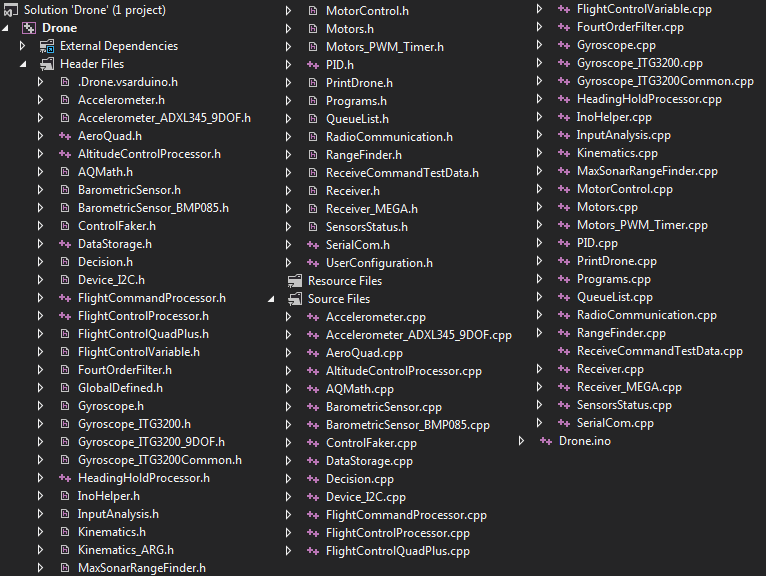
\includegraphics[width=\textwidth]{CodeOverviewDrone}
\caption{Overblik for filer til dronen}
\label{Fig:CodeOverviewDrone}
\end{figure}


Når projektet er åbent vælges fra menuen:
\begin{itemize}
\item Tools $\rightarrow$ Visual Micro $\rightarrow$ Boards $\rightarrow$ Arduino Mega 2560 or Mega ADK
\item Tools $\rightarrow$ Visual Micro $\rightarrow$ Programmer $\rightarrow$ AVRISP mkII
\item Tools $\rightarrow$ Visual Micro $\rightarrow$ Serial Port $\rightarrow$ COM? (der er et spørgsmålstegn, for nummeret afhænger af, hvilken port USB-kablet er isat).
\end{itemize}

Herefter er projektet klar til at blive kompileret og kørt.
Foretag et Build, eller vælg menuen Debug $\rightarrow$ Start Debugging for at overføre programmet til dronen.


\subsubsection{Sender og modtager}
For at downloade af projekt filerne, se afsnit \ref{sec: Drone}.

For at programmere sender og modtager bruges Atmel Studio 6. 6.1\footnote{\url{http://www.atmel.com/tools/atmelstudio.aspx}} 

Inde i Modtager/Sender mapperne er der filer der slutter på ".atsln". Disse filer er projektfilerne til koden. Hvis disse filer åbnes, starter projektet op hvis man har Atmel Studio installeret.

For at kompilere, i menuen i toppen trykkes på;
\begin{itemize}
\item Build $\rightarrow$ Bulid Solution.
\end{itemize}

For at programmere;
Først skal der tilføjes et target (det kan eks. være et STK500 Kit). Det gøres ved at trykke på;
\begin{itemize}
\item Tools $\rightarrow$ Add target.
\end{itemize}
For selve programmeringen;
\begin{itemize}
\item Tools $\rightarrow$ Device Programming $\rightarrow$ Vælg Tool og Device $\rightarrow$ Tryk Apply $\rightarrow$ I venstre side vælges Memories $\rightarrow$ i flash vælges filen der skal flashes (Ligger normalt under debug i projektmappen og slutter på elf) $\rightarrow$ Tryk Program
\end{itemize}

Når sender projektet åbnes, skulle filerne på Figur \ref{Fig:CodeOverviewSender} gerne vises i Solution Explorer.

\begin{figure}[H]
\centering
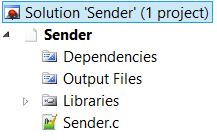
\includegraphics[scale=1]{CodeOverviewSender}
\caption{Overblik for filer til Senderen}
\label{Fig:CodeOverviewSender}
\end{figure}

Når Modtager projektet åbnes, skulle filerne på Figur \ref{Fig:CodeOverviewModtager} gerne vises i Solution Explorer.

\begin{figure}[H]
\centering
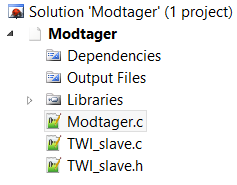
\includegraphics[scale=1]{CodeOverviewModtager}
\caption{Overblik for filer til Modtageren}
\label{Fig:CodeOverviewModtager}
\end{figure}


\end{document}